
%(BEGIN_QUESTION)
% Copyright 2012, Tony R. Kuphaldt, released under the Creative Commons Attribution License (v 1.0)
% This means you may do almost anything with this work of mine, so long as you give me proper credit

Skygg området/-ene i dette diagrammet som representerer følgende integral (forutsatt at hver horisontale og vertikale inndeling i diagrammet har trinnverdi 1):

$$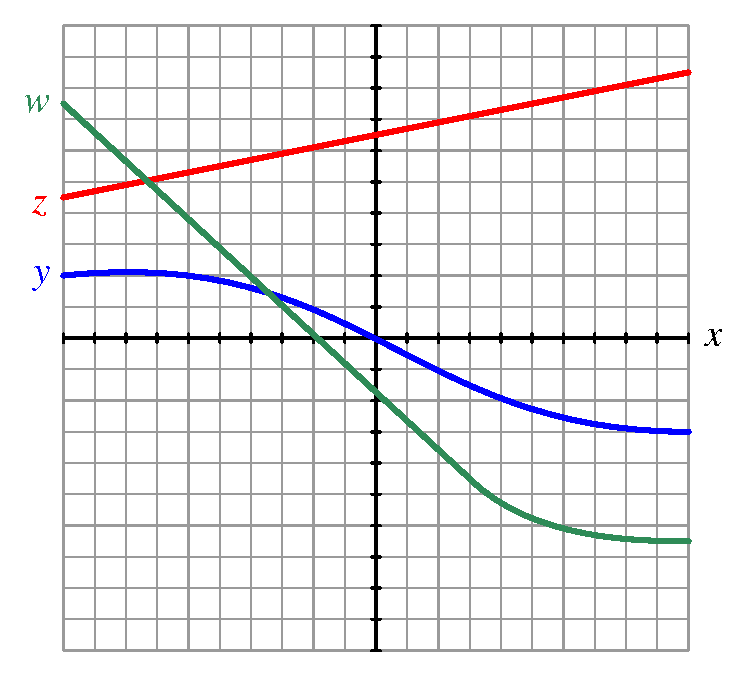
\includegraphics[width=15.5cm]{i01343x01.eps}$$

$$\int_{-6}^{3} (w - y) \> dx$$

Avgjør også om den numeriske verdien av dette integralet er {\it positiv} eller {\it negativ}.

\underbar{file i01343}
%(END_QUESTION)





%(BEGIN_ANSWER)

Dette integralet har en {\it negativ} verdi:

$$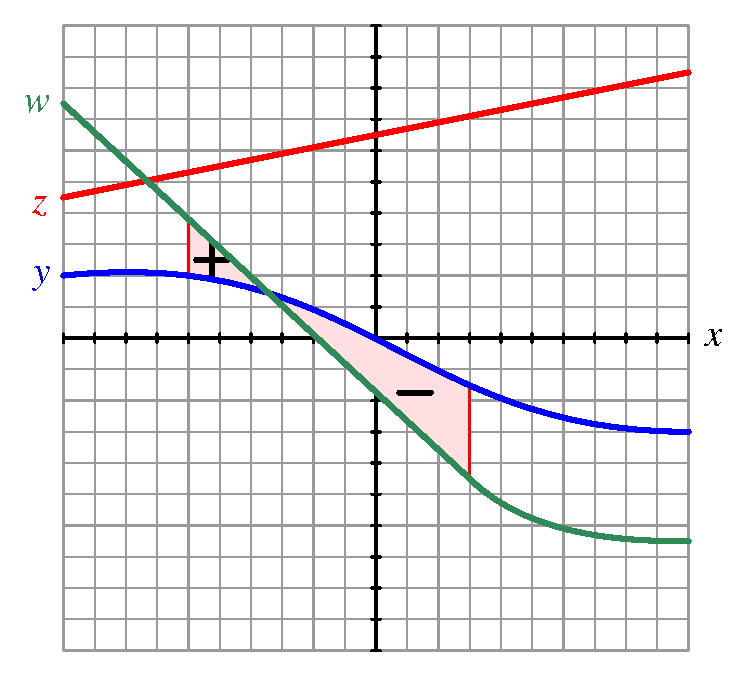
\includegraphics[width=15.5cm]{i01343x02.eps}$$

Fra $x = -6$ til omtrent $x = -3.5$ akkumulerer integralet en positiv verdi fordi $dx$-økningene er positive og $w$ er større enn $y$. Fra omtrent $x = -3.5$ til $x = 3$ akkumulerer integralet en negativ verdi fordi $y$ er større enn $w$ (negativ integrand), mens $dx$-økningene fortsatt er positive. Totalt er det negative arealet større enn det positive arealet, og derfor får integralet fra $x = -6$ til $x = 3$ en netto negativ verdi.

%(END_ANSWER)





%(BEGIN_NOTES)


%INDEX% Mathematics, calculus: integral (defined in a graphical sense)

%(END_NOTES)

